\chapter{Experimental Results}\label{chapter:results}

\begin{figure}[ht!]
    \centering
    \includegraphics[width=\textwidth]{thesis_latex_template/pics/accuracies_combined.png}
    \caption[Accuracies]{Average accuracy for the 16 models per coupling ratio $\rho$ in watermark scenario (top) and pattern scenario (bottom). left: on biased training data, right: on selection going against bias. As expected, for ellipses without watermark and rectangles with watermark, the accuracy drops as $\rho$ raises.}
    \label{fig:accuracy}
\end{figure}

In the following we summarize our findings for the experimental framework we constructed. We will firstly look at the model's reaction and ground-truth importance ($m_1)$, then visualize and describe the results for all explanation importance measures $m_2$.
Mostly we show plots for the first experiment, where the coupling ratio $\rho$ controls which images have an additional watermark. In cases where the outcome differs considerably to the scenario, where $\rho$ controls an overlapping pattern feature, we will also show and compare the results for this second benchmark. Further plots for the pattern scenario can be found in the appendix \cref{appendix:pattern_scenario}.

\section{Trained Models}
Here we report the training accuracies for the watermark and pattern scenario. 
As already noted in the method section, the model architecture is minimal but still has fairly high performance for the simple benchmark problems we test it on. 
For the watermark scenario the average performance is above 95\% and seems to be mostly independent from the coupling ratio $\rho$ as is visible in \cref{fig:accuracy} (left).
However, with closer inspection of the accuracies in the second scenario \cref{fig:accuracy} (bottom), there is a cut-off where the models start to rely solely on the spurious feature at $\rho \sim 0.8$, from which point the accuracy seems completely correlated with the presence of the spurious feature, i.e., with $\rho$.

A first impression on how much the coupling ratio $\rho$ affects the performance for instances that go against its bias, i.e., $W=0$ when $S=1$ and vice versa, can be seen in \cref{fig:accuracy} (right). We will in the following examine this reaction of the model in more detail with the measures for ground-truth relative feature importance $m_1$ discussed in the method \cref{section:gt_measure}. 

In \cref{fig:m0_m1} the relationship between the causal variable $\rho$ and the distribution within our dataset is compared to the models reaction. Because the causal variables $S$ and $W$ are binary, their correlation is not exactly following the linear increase of $\rho$ but starts of slightly slower. Yet, the models feature importance is not linear to either this data-correlation nor to $\rho$.

\begin{figure}[t!]
\centering
    \includegraphics[height=4.42cm]{thesis_latex_template/pics/m1_m0_shape.png}
    \includegraphics[height=4.42cm]{thesis_latex_template/pics/m1_m0_shape_overlap.png}
    \caption[$m_0$ vs. $m_1$]{Comparing correlation in training data distribution biased by $\rho$ with the biased models reaction (prediction flip and mean logit change) to an unbiased subset of 6400 images. left: watermark scenario, right: pattern scenario }
    \label{fig:m0_m1}
\end{figure}

Instead, the models seem to mostly ignore the spurious feature until the correlation becomes quite high (watermark $\sim 0.9$, pattern $\sim 0.8$). Then, a state change  occurs and the spurious feature takes over rapidly. As a complementary view, one can observe the dependency between the target feature shape ($S$) and the prediction ($Y$) deteriorate accordingly when the spurious feature is coupled strongly. For the watermark scenario on average the correlation between $W$ and $Y$ never becomes higher than the to-be-learned correlation between $S$ and $Y$. In the appendix we additionally report the dependencies for the other latent factors of the image generation process (scale, rotation, x- and y-position) \cref{fig:other_latents_reaction} as a baseline comparison.
Results for the pattern benchmark are generally following a similar trend, but the spurious feature seems to be harder to ignore for the pattern scenario. Consequently, for low values of $\rho$ the model importance is already significantly larger than zero. Adding to that, the model seems to ignore the true feature shape when the correlation between shape and pattern becomes circa 0.8 and follows $\rho$ approximately linearly after that. We hypothesize that this is due to the higher entanglement of pattern and shape. 

While all models seem to learn to ignore the spurious feature up until a correlation in the data distribution of about 0.8, some continue to mostly dismiss it as the correlation gets even stronger, while others start using mainly the spurious feature for prediction. Therefore we found it important to also show each set of models trained with the same random initialization (i.e. same set of initial weights and biases) separately (\cref{fig:gt_over_seeds}). We speculate this robustness to spurious features to be, because the local minimum around using the spurious feature in the gradient function is further (or harder to reach) from their initial point. It certainly is a phenomenon worth studying and multiple authors have set to explicitly de-biasing networks using e.g. adapted cost functions, adversarial methods or human-in-the-loop correction \citep{Anders2022,Pahde2023,Reimers2021, Reimers2021b, Dreyer2023a}.
Conversely, in the pattern scenario most models seem to react to the spurious feature stronger (as visible in \cref{fig:compare_seeds_overlap}). This is in line with the earlier hypothesis that this kind of spurious feature creates a harder-to-evade bias.  

\begin{figure}[t!]
    \centering
    \includegraphics[width=\textwidth]{thesis_latex_template/pics/compare_seeds.png}
    \caption[Comparing Seeds]{Mean logit change, prediction flip, accuracy over 16 random seeds.
    }
    \label{fig:gt_over_seeds}
\end{figure}

A second noteworthy observation one can make from the individual model view is that some seeds seem to be less stable in performance than others. Nevertheless no relationship between this instability and the models reaction to the spurious feature is apparent so we propose that those artifacts are not polluting the importance analysis. As suggested among others by \citet{Karimi2023} an explanations \textit{goodness} should not depend on the accuracy of the model it is explaining. 

\subsection{Ground Truth Model Importance $m_1$}
In the method section we described multiple distance metrics for measuring the effect of the spurious feature. It becomes apparent in \cref{fig:m1_results} that the choice of distance metric is not majorly changing the overall trend.
The prediction flip measure seems to almost coincide with its non-binarized analogue, the mean logit change, for the watermark case.
In the pattern scenario on the other hand, the prediction flip has a higher value than the mean logit change as soon as the spurious feature (the pattern) takes over. An explanation is that although the model starts to only use the pattern feature from that point on, its confidence on this decision is not as high as in the other case.

We show the absolute, squared and cosine distance of the logit vectors in the plot (\cref{fig:m1_results}), which all have similar curves. This is in order to identify how strongly they deviate and to potentially enable better comparison with the analogous $m_2$ measures.
In the method \cref{section:measure_mac} we introduced this multitude of distance metrics for the output logits, the relevance vectors and the attribution maps. The cosine distance measure proves to be not only straight-forward to implement because it does not necessitate normalization prior to its application but also yields highly correlated results to the other measures. 
Prior work on comparing relevance vectors also mostly uses cosine similarity or related metrics \citep{Sixt2020, Achtibat2022,Achtibat2023, Dreyer2023a}, which is why we focus on its results looking forward.  
In \cref{appendix:distance_metrics} the other distance metrics are analyzed for completeness.

\begin{figure}[t!]
    \centering
    \includegraphics[height=5.75cm]{thesis_latex_template/pics/m1_main_comparison.png}
    \includegraphics[height=5.75cm]{thesis_latex_template/pics/m1_main_comparison_overlap.png}
    \caption[Ground Truth Importance $m_1$]{Ground truth model importance $m_1$: mean logit change (MLC) with different distance metrics and prediction flip}
    \label{fig:m1_results}
\end{figure}

\section{Explanation Importance}

\begin{figure}[t!]
    \centering
    \includegraphics[height=5.75cm]{thesis_latex_template/pics/m2_cosine_comparison.png}
    \includegraphics[height=5.75cm]{thesis_latex_template/pics/m2_cosine_comparison_overlap.png}
    \caption[Relevance Vectors and Attribution Maps, Comparison of Metrics]{Comparison of distance metrics for relevance vectors (of 8 concepts in last convolutional layer) and attribution maps (each with dimension 64x64).}
    \label{fig:m2_cosine_comparison}
\end{figure}

Next we compare the effect of the coupling variable $\rho$ on the ground truth model importance $m_1$ to the explanation importance $m_2$. 
If the explanation importance strongly deviates from the true spurious feature importance, it would mean that the explanation is not able to recover and explain spurious features sufficiently. Though as hinted at in the formulation of the measures, it is not evident how to scale each measure. Without the ground truth available, there are no other values of feature importance one can relate the case at hand to. We still attempt to define the measures' outputs such that if an explanation solely explains based on the spurious feature, the metric has the value 1. 
Another way to make the measures comparable in growth would be to scale each of them to the [0,1] interval. We believe that this would not be in line with how our framework is defined. The model importance does not exceed $\sim 40$ percent on average in the first scenario, while almost reaching $100$ percent in the other. Furthermore, measures like \textit{RMA} are unlikely to actually reach 1 and scaling the measure would not yield sensible results. Instead, we define each measures scaling individually, to assure that its full extent also lies within the [0,1] interval.
We show the curves in relation to $\rho$ to gain insight into this relationship. However, as we will see later, the models reaction to the spurious feature is not always in line with $\rho$. Hence it is also insightful to look at the direct relationship between $m_1$ and $m_2$ measures through scatter plots for some particular examples.

\subsection{Relevance Vectors and Attribution Maps Importance}
Firstly we show the causal effect of intervention on $W$ in relation to $\rho$ on the relevance vectors and their respective attribution images. 
The relevance vectors are the normalized absolute sums of the respective attribution maps. Therefore it is not surprising that the two types of measures produce related results.
These distance metrics mostly follow the general trend of the true model importance for the watermark scenario (see \cref{fig:m2_cosine_comparison} left). In the pattern scenario (\cref{fig:m2_cosine_comparison} right), the overall trend still stays the same but both the relevances and their respective attribution maps are less strongly coupled to $\rho$. While the importance of $W$ is overestimated when $\rho$ is in the low \textit{state}, it is underestimated where the pattern feature is used exclusively by the models. A similar observation can be made for most other measures for the pattern scenario. 


\subsection{Region-Specific Importance}

\begin{figure}[ht!]
\centering
    \includegraphics[height=5.75cm]{thesis_latex_template/pics/m2_region_both_comparison.png}
    \includegraphics[height=5.75cm]{thesis_latex_template/pics/m2_region_both_comparison_overlap.png}
    \caption[Region Specific, Comparison of Metrics]{Comparison of distance metrics using bounding box of spurious feature. solid lines: weighted sum, dashed lines: most relevant neuron}
    \label{fig:m2_region_comparison}
\end{figure}

The measures using the boundary around the watermark feature to establish its relative importance are following the true model importance less closely (see \cref{fig:m2_region_comparison}). 
This in turn means that some of the effect of intervening on the spurious feature, i.e. adding or removing the watermark, changes the attribution maps in regions other than the watermark region. We show the aggregated measures both for the weighted sum of all concepts and for only the most relevant concept. 
In the watermark scenario $\RMA$ and $\RRA$ are more accurate at assigning no importance to the spurious feature region when $\rho$ is low. But the area never gets as much explained importance as the model applies to the feature when $\rho$ is high. Instead, as can be seen from closer inspection of example attribution maps \cref{fig:example_relchange_outside_wm}, the difference is also expressed through changing relevance in the background or shape. 
The simplified $\PG$ measure, especially the version which aggregates all concepts' measurements, overestimates the feature importance of the watermark for all values of $\rho$. Especially for high $\rho$ where the true importance is still quite low it deviates considerably.

\begin{figure}[t!]
    \centering
    watermark: relevance change outside of watermark region\\
    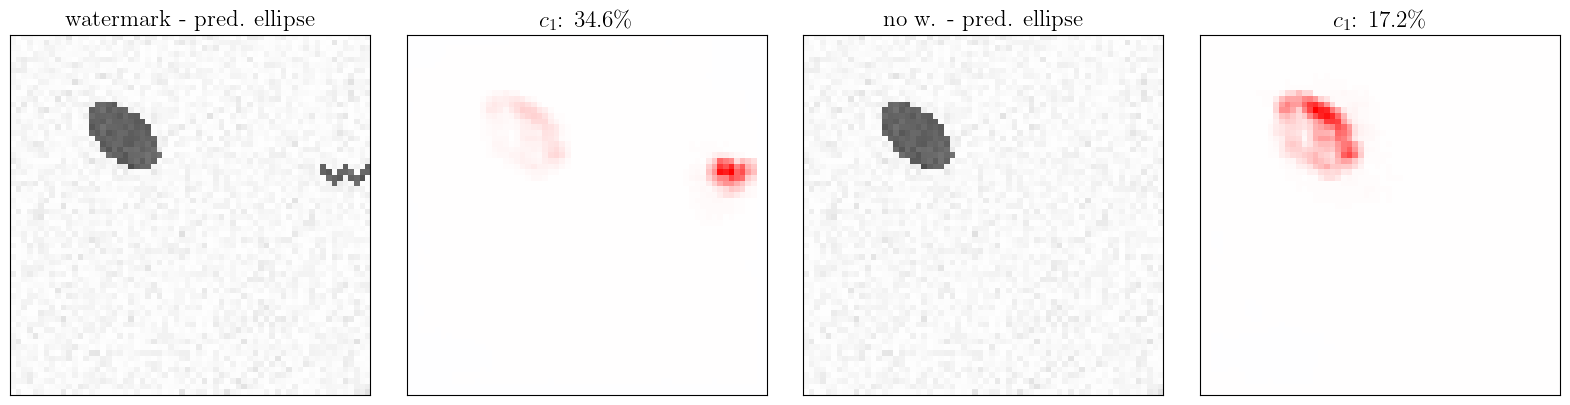
\includegraphics[width=0.9\linewidth]{thesis_latex_template/pics/example_relchange_outside_wm.png}\\
    pattern: zero relevance when ``wrong'' pattern\\
    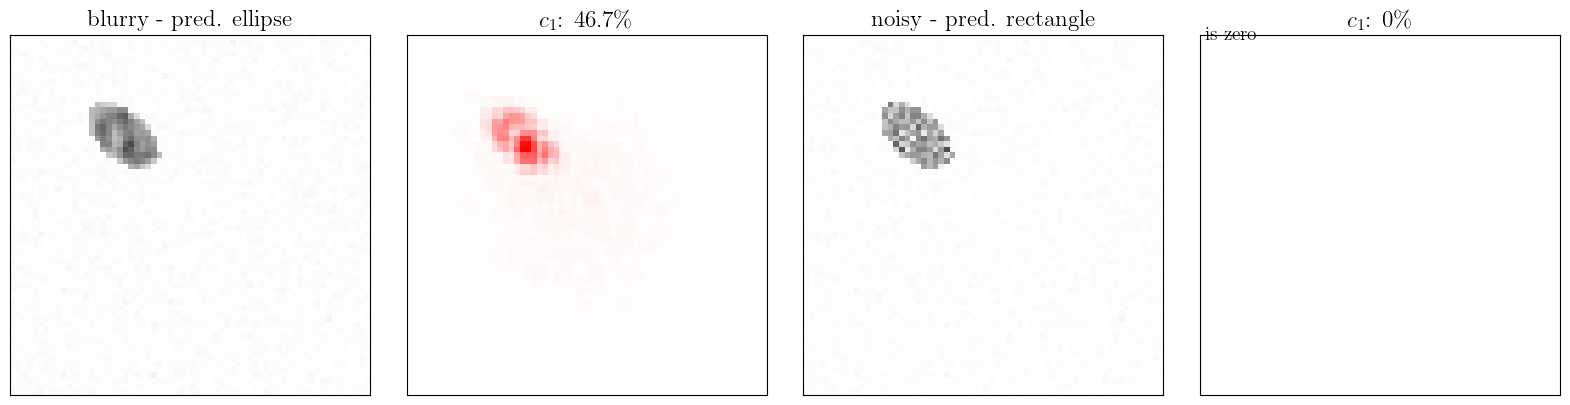
\includegraphics[width=0.9\linewidth]{thesis_latex_template/pics/example_relchange_pattern.png}\\
    pattern: top neurons $c_1, c_0$ have similar heatmaps but encode different patterns\\
    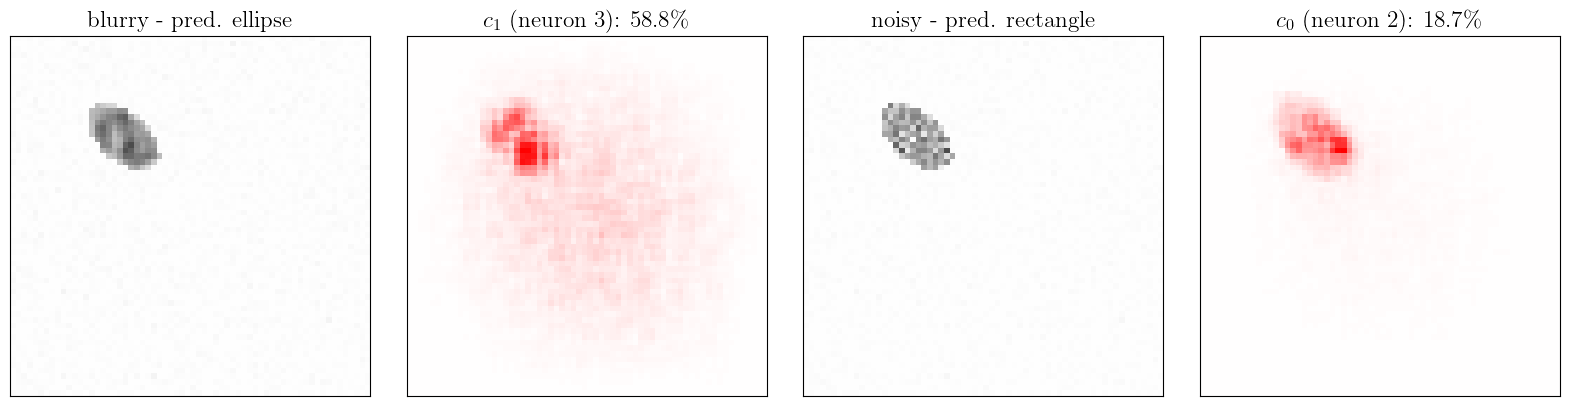
\includegraphics[width=0.9\linewidth]{thesis_latex_template/pics/example_top_neuron_broken.png}
    \caption{Examples of heatmaps for highly biased neurons (of models that only use the spurious feature for prediction). }
    \label{fig:example_relchange_outside_wm}
\end{figure}

Surprisingly, the curves of the region-specific measures more or less follow the ground truth for the pattern scenario as well. When looking at heatmaps for a highly biased neuron for a shape with the noisy and blurry pattern, the reason becomes clear (see second row \cref{fig:example_relchange_outside_wm}): If a neuron exclusively encodes a pattern (noisy or blurry), it assigns zero relevance to the same shape with the opposing pattern. Although the $\PG$ measure underestimates the feature importance at all times, likely because the most important pixel almost always lies within the shape boundary, this effect is also slightly visible for high $\rho$. 
Yet, the region-specific measures when using the top neurons difference of the blurry and noisy images ($c_1- c_0$)  are growing less with the ground truth importance here. The last row of \cref{fig:example_relchange_outside_wm} gives an intuition for that: If the top concept is selected for either image separately, one will assign relevance within the boundary because of the noisy-ness, and the other because of the blurry-ness of the respective image. Their difference is therefore not large. 

\section{Relevance Maximization Reference Sets Importance}
\begin{figure}[ht!]
    \centering
    \includegraphics[height=5.75cm]{thesis_latex_template/pics/m2_refset_comparison.png}
    \includegraphics[height=5.75cm]{thesis_latex_template/pics/m2_refset_comparison_overlap.png}
    \caption[Reference Sets, Comparison of Metrics ]{Comparison of distance metrics using the prototypical reference sets. Here: maximizing summed relevance per image }
    \label{fig:m2_refset_relevance}
\end{figure}
The measures listed before have shown that the explanation produced with concept-conditional attribution maps to some degree uncovers the true relative importance of a spurious feature.
In the watermark case most $m_2$ values are reasonably close to the true model importance's curve.
However, the pattern scenarios results are less convincing. As mentioned in previous chapters, we constructed a measure aiming to evaluate how reference sets for neurons can alleviate some of the weaknesses of local attribution maps for spatially overlapping features. 

In the following we summarize the results for our metrics using the relevance maximization reference sets, which ought to reveal \textit{what} a concept encodes. \Cref{fig:m2_refset_relevance} compares the results for the general reference sets and the class-specific reference sets. 
The $\SPF$ measure, using the non-class-specific reference sets, is able to follow the ground truth importance, though more noisily than previous measures. 
Albeit some effect is visible for the class-specific measure $\YSPF$ too, it underestimates the importance of the spurious feature for highly coupled instances considerably. For the highest coupling ratios the value is even decreasing. 
When looking at some example reference sets (\cref{fig:class_reference_sets}), possible reasons become visible: The most important concepts for either class actually seem to not be consistent about the pattern. While $c_2$ is very important for the rectangle, the pattern is equally noisy or blurry in the reference set. The opposite occurs for concept $c_7$. The relevances for either class of these two concepts give us the hint that the measure might not work as expected because of how negative relevance is dealt with. For example, $c_2$ has strong negative relevance for the ellipse shape, even though it seems to encode blurry ellipses. Yet, for the rectangle shape it is most important but seems to not encode the noisy pattern. Our assumption is that the concept could be interpreted as \textit{not-blurry}, but the way we measure $\YSPF$ can not identify such a negative concept.

% reference set: bias: 1.0, num_it = 7, concepts 7,4,6,0
% also interesting: [2,5,7], bias 1.0, num_it 11
\begin{figure}[t!]
    \centering
    \includegraphics[width=0.8\linewidth, angle=-90]{thesis_latex_template/pics/example_stats_relevances.png}
    \caption{Examples of class specific reference sets for top-3 important neurons ($c_2, c_5, c_7$) of highly biased model (seed 11, bias 1.0). We are only showing a subset of the 6 top images for each class $s_0$ (rectangle) and $s_1$ (ellipse).}
    \label{fig:class_reference_sets}
\end{figure}

\subsection{Activation versus Relevance Maximization}
\begin{figure}[ht!]
    \centering
    \includegraphics[height=4.6cm]{thesis_latex_template/pics/m2_refset_rva_comparison.png}
    \includegraphics[height=4.6cm]{thesis_latex_template/pics/m2_refset_rva_comparison_overlap.png}
    \caption[Reference Sets, Relevance/Activation, Sum/Max ]{
    Comparison of $\SPF$ using different maximization targets (sum/max) and relevance or activation, when distribution of shape is taken into account.
    }
    \label{fig:m2_refset_rel_vs_act}
\end{figure}

In their paper, the authors of CRP find that relevance maximization is better able at showing a concept in the context it is most often used in \citep{Achtibat2022}.
While this might help humans in understanding the concept within the given context, it also correlates other features with the concept's main feature. This makes it harder to decide which of all the correlated features the concept actually encodes, we refer to \cref{fig:m2_refset_rel_vs_act} for examples on this (also earlier images \cref{fig:act_rel_max,fig:entangled_ref_set}).
We hence incorporated the distribution of the shape feature into our measure using a variation of $\SPF$ with a relative spurious feature share $\RE^{relative}$ (see \cref{eq:re_relative}).
This way, reference sets are penalized when all images within them not only share the pattern but also share the shape. 
For this measure the values are lower on average, as only an unbiased distribution of shapes within the reference sets is interpreted as high relevance for the pattern feature. A reference set with, e.g., only blurry ellipses would have feature importance 0.5, while if it would have blurry rectangles and blurry ellipses in equal parts, it would have assign perfect importance to the blurry pattern. 

Since the activation maximization reference sets do not show the concept \textit{in its context} as much, they have higher values for $\SPF$ and $\YSPF$ \cref{fig:m2_refset_rel_vs_act}. 
In accordance with the observations from \cite{Achtibat2022}, using the summed relevance of an image as the maximization target is more robust and also performs better for our measures than using the maximal relevance. 

\section{Quantitative Comparison}
After having visually analyzed the results we here summarize the findings using a table. Our experiment has essentially intervened on the spurious feature $W$ and the coupling ratio $\rho$. The curve of ground truth measure $m_1$ thereby shows the causal effect of intervention on $\rho$ on the model importance of $W$. On the other hand, the explanation metrics $m_2$ show the causal effect of this intervention on the explanations' importance of the spurious feature. 
While the perspective of a mean curve 

Could just use correlation as a measure? mean squared error etc. is probably not the best idea.

\begin{table}[!ht]
    \centering
    \begin{tabular}{l|ll|ll}
    \hline
        \textbf{measure}& \textbf{watermark} R2 &  & \textbf{pattern} R2 &  \\ \hline
        & $\rho$ & \textbf{seed} & $\rho$  & \textbf{seed} \\ \hline
        RelVec. Absolute & 0.95 & 0.91 & 0.99 & 0.85 \\ \hline
        RelVec. Cosine & 0.96 & 0.9 & 0.98 & 0.64 \\ \hline
        Attr. Absolute & 0.95 & 0.89 & 0.95 & 0.73 \\ \hline
        Attr. Cosine & 0.95 & 0.88 & 0.98 & 0.69 \\ \hline
        $\RMA$ weighted & 0.96 & 0.76 & 0.96 & 0.45 \\ \hline
        $\RMA$ $c_1- c_1$ & 0.98 & 0.81 & 0.94 & 0.35 \\ \hline
        $\RMA$ $c_1- c_0$ & 0.98 & 0.82 & 0.94 & 0.4 \\ \hline
         $\PG$  weighted & 0.83 & 0.61 & 0.81 & 0.09 \\ \hline
         $\PG$  $c_1- c_1$ & 0.92 & 0.7 & 0.61 & 0.06 \\ \hline
         $\PG$  $c_1- c_0$ & 0.92 & 0.71 & 0.59 & 0.08 \\ \hline
        $\RRA$ weighted & 0.97 & 0.77 & 0.98 & 0.78 \\ \hline
        $\RRA$ $c_1- c_1$ & 0.98 & 0.8 & 0.97 & 0.67 \\ \hline
        $\RRA$ $c_1- c_0$ \$W\$ & 0.98 & 0.8 & 0.93 & 0.37 \\ \hline
        RelMax sum general & 0.89 & 0.46 & 0.96 & 0.53 \\ \hline
        RelMax sum penalize shape & 0.89 & 0.44 & 0.96 & 0.52 \\ \hline
        RelMax sum per class & 0.73 & 0.27 & 0.67 & 0.09 \\ \hline
        ActMax sum general & 0.84 & 0.32 & 0.98 & 0.55 \\ \hline
        ActMax sum penalize shape & 0.86 & 0.29 & 0.98 & 0.58 \\ \hline
        ActMax sum class & 0.86 & 0.38 & 0.98 & 0.58 \\ \hline
    \end{tabular}
    \caption{R2 (correlation coefficient) between cosine mean logit change $m_1$ and evaluated measures $m_2$, for watermark and pattern scenario. Once over mean per step of $\rho$ and once per model (seed)}
\end{table}


\begin{table}[!ht]
    \centering
    \begin{tabular}{l|ll|ll}
    \hline
        \textbf{measure}& \textbf{watermark} &  & \textbf{pattern} &  \\ \hline
        & $\rho$ & \textbf{seed} & $\rho$  & \textbf{seed} \\ \hline
        RelVec. Absolute & 0.00072 & 0.0022 & 0.00721 & 0.0163 \\ 
        RelVec. Cosine & 0.00033 & 0.0015 & 0.00984 & 0.0268 \\ 
        Attr. Absolute & 0.00064 & 0.0016 & 0.01115 & 0.0233 \\ 
        Attr. Cosine & 0.00033 & 0.0021 & 0.01193 & 0.0256 \\  \hline
        $\RMA$ weighted & 0.00228 & 0.0031 & 0.01152 & 0.0489 \\ 
        $\RMA$ $c_1- c_1$ & 0.00156 & 0.0023 & 0.01445 & 0.0606 \\ 
        $\RMA$ $c_1 - c_0$ & 0.00157 & 0.0023 & 0.05888 & 0.0676 \\ 
        $\PG$ weighted & 0.00622 & 0.0135 & 0.07339 & 0.1031 \\ 
        $\PG$ $c_1- c_1$ & 0.00153 & 0.0062 & 0.07247 & 0.104 \\ 
        $\PG$ $c_1 - c_0$ & 0.00154 & 0.0063 & 0.06315 & 0.098 \\ 
        $\RRA$ weighted & 0.00181 & 0.0027 & 0.01134 & 0.0181 \\ 
        $\RRA$ $c_1- c_1$ & 0.00078 & 0.0024 & 0.01311 & 0.026 \\ 
        $\RRA$ $c_1 - c_0$ & 0.00078 & 0.0024 & 0.05251 & 0.0664 \\  \hline
        RelMax sum general & 0.00076 & 0.0118 & 0.00751 & 0.0612 \\ 
        RelMax sum penalize shape & 0.00147 & 0.012 & 0.04432 & 0.0613 \\ 
        RelMax sum per class & 0.00255 & 0.0091 & 0.08671 & 0.1145 \\ 
        ActMax sum general & 0.00197 & 0.0116 & 0.00723 & 0.0601 \\ 
        ActMax sum penalize shape & 0.00258 & 0.0102 & 0.01854 & 0.0503 \\ 
        ActMax sum per class & 0.00222 & 0.009 & 0.00804 & 0.0561 \\ \hline
    \end{tabular}
    \caption{Mean Squared Error (MSE) between cosine mean logit change $m_1$ and evaluated measures $m_2$, for watermark and pattern scenario. Once over mean per step of $\rho$ and once per model}
\end{table}